\documentclass[11pt]{article}
\usepackage{mathpazo}
\usepackage{url}
\usepackage{verbatim}
\usepackage{graphicx}

\newcommand*{\prg}{\textsc{Erigone}}
\newcommand*{\eui}{\textsc{EUI}}
\newcommand*{\spn}{\textsc{Spin}}
\newcommand*{\jsp}{\textsc{jSpin}}
\newcommand*{\prm}{\textsc{Promela}}
\newcommand*{\p}[1]{\texttt{#1}}
\newcommand*{\bu}[1]{\textsf{#1}}

\textwidth=15cm
\textheight=22.5cm
\topmargin=0pt
\headheight=0pt
\oddsidemargin=1cm
\headsep=0pt
\renewcommand{\baselinestretch}{1.1}
\setlength{\parskip}{0.20\baselineskip plus 1pt minus 1pt}
\parindent=0pt

\title{The \eui{} Development Environment for the\\
\prg{} Model Checker\\Quick Start Guide}
\author{Mordechai (Moti) Ben-Ari\\
Department of Science Teaching\\
Weizmann Institute of Science\\
Rehovot 76100 Israel\\
\textsf{http://stwww.weizmann.ac.il/g-cs/benari/}}
%\date{}
\begin{document}
\maketitle
\thispagestyle{empty}

\vfill

\begin{center}
Copyright \copyright{} 2010-12 by Mordechai (Moti) Ben-Ari.
\end{center}
This work is licensed under the Creative Commons Attribution-ShareAlike 3.0
License. To view a copy of this license, visit
\url{http://creativecommons.org/licenses/by-sa/3.0/}; or, (b) send a letter
to Creative Commons, 543 Howard Street, 5th Floor, San Francisco,
California, 94105, USA.

\newpage

\section{Introduction}

\prg{} is a \emph{model checker} that can simulate and verify concurrent
and distributed programs. It is a partial reimplementation of the \spn{}
model checker and supports a large subset of \prm{}, the modeling language
used by \spn{}. \eui{} is a development environment for \prg{} that
includes a graphical user interface and algorithms to format and display
the result of a simulation and verification. \eui{} is an adaptation of the
\jsp{} development environment for \spn{}.

There are comprehensive User's Guides and software documentation for
both \prg{} and \eui{}. This document is intended to be a quick
introduction to working with \prg{} using the \eui{} environment.

The \prg{} and \eui{} software are copyrighted under the \textsc{GNU}
General Public License. The copyright statement and the text of the
license are included in the distribution.

Introductory textbooks on concurrency and model checking are:

\begin{itemize}
\item M. Ben-Ari. \textit{Principles of Concurrent and Distributed Programming (Second
Edition)}. Addison-Wesley, 2006.
\item M. Ben-Ari. \textit{Principles of the Spin Model Checker}.
Springer, 2008.
\end{itemize}

\textbf{Acknowledgment:}\\I would like to thank for H. Peter Gumm for
his comments on this guide.

\section{Installation and execution}

This section describes the installation and execution of \eui{} and \prg{}
under the Windows operating system. For other systems, see the User's Guides.

\eui{} needs the Java JRE, version 1.5 at least. 

Download the \eui{} installation file \p{eui-N.exe} (where \p{N} is the
latest version number) from the \jsp{} project at Google Code
\url{http://code.google.com/p/jspin/} and execute the installation file.
The installation contains the executable file for
\prg{} so you don't need to install it separately.

By default, an icon to run \eui{} is installed on the Desktop. If Java
is associated with \p{jar} files, double-clicking on the icon will run
\eui{}. Click on \bu{Open} to open a \prm{} source file in the edit
window on the left.

The user interface of \eui{} is shown on the following page.

\begin{figure}[tb]
\begin{center}
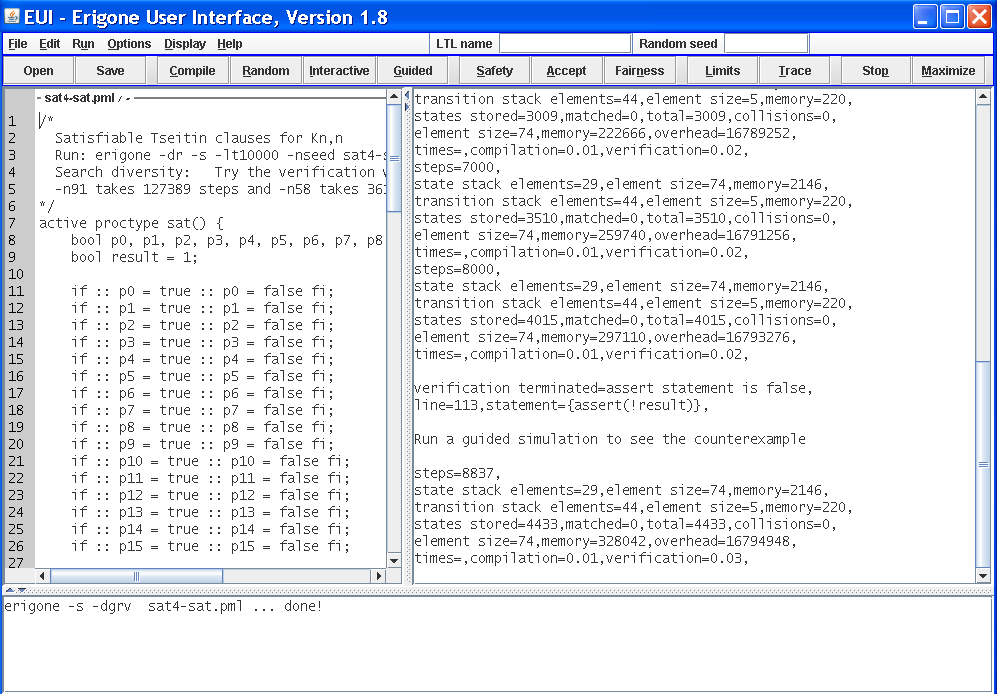
\includegraphics[width=120mm]{eui}
\end{center}
\end{figure}


\section{Simulating a \prm{} program}

This section show how to simulate two \prm{} programs for the mutual
exclusion problem; the first has an error that causes mutual exclusion
to be violated, whereas mutual exclusion always holds in the second
program.

\subsection*{The Second Attempt}

The first program is the Second Attempt to solve the mutual
exclusion problem (Ben-Ari, 2006, Section~3.6) and is contained in
the file \p{second.pml} in the \p{examples} directory:

\begin{verbatim}
bool wantp = false, wantq = false;
byte critical = 0; 

active proctype p() {
    do 
    :: !wantq;
       wantp = true;
       critical++;
       assert (critical == 1);
       critical--;
       wantp = false;
    od
}

active proctype q() { /* Symmetrical */ }
\end{verbatim}

Open the file \p{second.pml} in the \p{examples} directory. The \prm{}
source code will be displayed in the left-hand pane. Click on
\bu{Random} to run a simulation. The result will be something like:

\pagebreak[4]

\begin{verbatim}
Erigone v2.1.3, Copyright 2008-9 by Moti Ben-Ari, GNU GPL.
execution mode=simulation,
simulation mode=random,seed=-1,trail number=0,total steps=10,

Process Statement            critical      wantp      wantq 
q       19 !wantp                   0          0          0 
p        7 !wantq                   0          0          0 
q       20 wantq = true             0          0          0 
p        8 wantp = true             0          0          1 
p        9 critical++               0          1          1 
q       21 critical++               1          1          1 
q       22 assert (critica          2          1          1 

simulation terminated=assert statement is false,
line=22,statement={assert (critical == 1)},

steps=7,
times=,compilation=0.01,simulation=0.01,
\end{verbatim}

The states of the simulation are displayed in tabular form similar to
that used in Ben-Ari (2006). The first column is the process from which
a statement was executed; the next column contains the line number and
source code of the statement; the rest of the columns give the values of
the variables in the state. Following the table, the result of the
simulation is given. Since \p{critical} has the value~2 when the assert
statement in line~22 of the program is evaluated, an error has occurred
and the simulation terminates.

The tabular display of the scenario is created by the \eui{} software
from the output of \prg{}. The other information is displayed in the raw
format used by \prg{}: comma-terminated named associations of the form
\p{"name=value,"}.

\subsection*{Mutual exclusion with a semaphore}

The second program uses a semaphore to achieve mutual exclusion
and is contained in the file \p{sem.pml} in the \p{examples} directory:

\pagebreak[4]

\begin{verbatim}
byte sem = 1;
byte critical = 0;

active proctype p() {	
  do :: 
    atomic {
      sem > 0;
      sem--
    }
    critical++;
    assert(critical == 1);
    critical--;
    sem++
  od
}

active proctype q() {	/* The same */ }

active proctype r() {	/* The same */ }	
\end{verbatim}

Open the file \p{sem.pml} and click \bu{Random}. Since no error is
encountered the states of the simulation will be displayed for a very
long time (until a step count limit is reached). Click \bu{Stop} to stop
the simulation prematurely.

These simulations were \emph{random simulations}, where the
(nondeterministic) selection of the next statement to execute is chosen
randomly. See the User's Guide for information on how to run an
\emph{interactive simulation} where you control the section of
statements. \emph{Guided simulation} is explained in the next section.

\section{Verifying a \prm{} program with assert statements}

Open the file \p{second.pml} and click on \bu{Safety} to perform a
verification in \emph{Safety mode}. The result will be displayed in the
right-hand pane:
\begin{verbatim}
verification terminated=assert statement is false,
   line=22,statement={assert (critical == 1)},

Run a guided simulation to see the counterexample
\end{verbatim}

Click \bu{Guided} to run a \emph{guided simulation} using the trail
which describes the \emph{counterexample}, the sequence of states found
during the verification that leads to a violation of mutual exclusion.

Open \p{sem.pml} and click on \bu{Safety}. The result is as expected:
\begin{verbatim}
verification terminated=successfully,
\end{verbatim}

\section{Verifying a safety property using LTL}

\prg{} can verify a correctness property written as a formula in
\emph{linear temporal logic (LTL)}.
The program in the file \p{second-ltl.pml} is the same as that in
\p{second.pml} except that the assert statements have been removed
and an LTL formula has been added:
\begin{verbatim}
bool wantp = false, wantq = false;
byte critical = 0;

ltl { [](critical<=1) }

active proctype p() {
    do 
	  :: !wantq;
       wantp = true;
       critical++;
       critical--;
       wantp = false;
    od
}

active proctype q() { /* Symmetrical */ }
\end{verbatim}
Read the LTL formula as: the value of \p{critical} is \emph{always}
(\p{[]}) less than or equal to 1.

Click \bu{Safety} to perform a verification in Safety mode. The output
will be:

\begin{verbatim}
Erigone v2.1.0, Copyright 2008-9 by Moti Ben-Ari, GNU GPL.
execution mode=safety,error number=1,hash slots=22,state stack=2,
  location stack=3,progress steps=1,total steps=10,

verification terminated=never claim terminated,
line=9,statement={critical--},

Run a guided simulation to see the counterexample

steps=47,
  ...
times=,compilation=0.04,verification=0.06,
\end{verbatim}

The first lines give information about the configuration used to run the
verification. This is followed by the result of the verification. The
phrase \emph{never claim terminated} is a technical term used by the
model checker to report that an error has been found. Finally,
information on the performance of the model checker is displayed. The
counterexample can be displayed by running a guided simulation.
Running a verification for the program with the semaphore gives the
result that the verification was terminated successfully.

\section{Verifying a liveness property using LTL}

Consider the following program (file \p{fair1.pml}) which is a very
simple example used to demonstrate the concept of fairness:
\begin{verbatim}
byte n = 0;
bool flag = false;

ltl { <>flag }

active proctype p() {
  do
  ::  flag -> break;
  ::  else -> n = 1 - n;
  od
}

active proctype q() {
  flag = true
}
\end{verbatim}

If process \p{q} ever executes, it will set \p{flag} to \p{true} and
process \p{p} will then terminate, but in an unfair computation (where
\p{q} never executes) this may never happen. Let us now try to prove the
property \p{<>flag} meaning that \emph{eventually} \p{flag} becomes
true. 

Click on \bu{Accept} to perform a verification in \emph{Acceptance
mode}. In this mode, the model checker searches for an \emph{acceptance
cycle}, which is the technical term for an error in a verification of an
LTL formula containing \emph{eventually} (\p{<>}). The result is:

\begin{verbatim}
verification terminated=acceptance cycle,
line=7,statement={else -> n = 1 - n},

Run a guided simulation to see the counterexample
\end{verbatim}

Click on \bu{Guided} to conduct a guided simulation that demonstrates
the computation with the acceptance cycle that is a counterexample to
the correctness property.

Click on \bu{Fairness} to perform a verification in \emph{Acceptance
mode with weak fairness}. In this mode, only weakly fair computations
are candidates for acceptance cycles. In a weakly fair computation,
continually enabled transitions must eventually be taken. Since the
assignment statement \p{flag=true} is obviously continually enabled, it
must be taken. When the verification is run, the result is:

\begin{verbatim}
verification terminated=successfully,
\end{verbatim}

\end{document}
